%\section*{resultsIntro}


\newthought{Even}~though all of the computer program's bottle-necks are parallelized in \href{http://en.wikipedia.org/wiki/SPMD}{SPMD}, an application to more than a decade of high-resolution \SSH~data still requires patience (say $\order{1}$ - $\order{2}$ days \footnote{depending on the number of CPU's and their frequencies.}). The most time-consuming of steps is the numerically arduous part of subjecting each of the vast number of found contours \footnote{see \cref{fig:allEddies-aviIaviIIpop7II}.} to the filtering procedure as described in \cref{S:04}.
The total number of final analyses was hence limited and it was therefor critical to carefully choose which method/parameters to use in order to maximize the deducible insights from the results.
For best comparability of the results with each other it was decided to agree on one complete set of parameters as a basis (\cref{tab:fixparams}), which would then be altered at key parameters.

%%....................................F.I.G.U.R.E.............................................
\begin{marginfigure}
\includegraphics[width=\linewidth]{defl-age-aviI_shrunk2prepress}
\caption{\aviI: Baseline-shifted \textit{old} ($age > \SI{500}{day}$) tracks.}
\label{fig:defl-age-aviI_shrunk2prepress}
\end{marginfigure}
%%...................................F.I.G.U.R.E.............................................

\begin{itemize}
\setlength\itemsep{0mm}
\item 
The first run is an attempt to reproduce the results from \citet{Chelton2011}. The \SSH-data for this run is therefor that of the \AVI~ product.
This method will be called \MI.
\item
The second run (\MII) is equivalent, except that this time the alternative $\IQ$-based shape filtering method as described in \cref{filter:shape} and the slightly different tracking-filter as described in \cref{item:checkDynamicIdentity} are used. \MII~is then fed with 7-day time-step \POP~data as well.
\item
To investigate what role spatial resolution plays, the \POP~data was remapped to that of the \AVI~data and fed to the \MI~method.
\item
Finally, to investigate the effects of resolution in time, an \MII-2-day-time-step run over \POP~data was executed. For its results and discussion see \cref{sec:downsampled}.
\item
Start and end dates were fix for all runs as the intersection of availability of both data sets.
\end{itemize}

%%....................................F.I.G.U.R.E.............................................
\begin{marginfigure}
\includegraphics[width=\linewidth]{defl-age-aviII_shrunk2prepress}
\caption{\aviII: (same as \cref{fig:defl-age-aviI_shrunk2prepress})}
\label{fig:defl-age-aviII_shrunk2prepress}
\end{marginfigure}
%%....................................F.I.G.U.R.E.............................................
%%

\begin{scriptsize}
\begin{margintable}
	\begin{tabularx}{\textwidth}{|X|X|}
	\hline
	time frame &  \displaydate{runsStart} till \displaydate{runsEnd}\\
	\hline
	scope & full globe ($80S:80N \;\; 180W:180E$) \\
	\hline
	\AVI geometry &   $641 x 1440$ true Mercator \\
	\hline
	POP   geometry &   $2400 x 3600$ \\
	\hline
	contour step   &   \contourstep \\
	\hline
	\end{tabularx}
	\begin{tabularx}{\textwidth}{|X|X|}
	\hline
	\textbf{thresholds} &  [all SI]  \\
	\hline
	max $\sigma/\Lr$ & \threshmaxRadiusOverRossbyL \\
	\hline
	min $\Lr$ & \threshminRossbyRadius \\
	\hline
	min $\IQ$ & \threshshapeiq \\
	\hline
	min number of data comprising found contour & \threshcornersmin \\
	\hline
	max(abs(Rossby phase speed)) & \threshphase \\
	\hline
		min amplitude & \threshamp \\
	\hline
	\end{tabularx}
	\caption{Fix parameters for all runs. \TODO{SI}}
\label{tab:fixparams}
\end{margintable}

%\newpage
%\begin{margintable}
	%\begin{tabularx}{1.1\textwidth}{|X||X|X|}
	%\hline
	 %& \MI & \MII   \\
	%\hline
%shape threshold & The distance between any pair of points within the connected region must be less than a specified maximum. & The Isoperimetric Quotient must be at least a specified minimum.\\
	%\hline
%Comparison of old to new eddy & ratio between new and old must lie between $0.25$ and $2.5$ for amplitude and area TODO ref & similar but with $\sqrt{\mathrm{area}/\pi}$ instead of area and the lower threshold as reciproke of the higher and vice versa.   TODO ref \\
	%\hline
	%\end{tabularx}
	%\caption{The two methods \MI and \MII.}
%\label{tab:MIMIIdiffs}
%\end{margintable}
\end{scriptsize}


\begin{infobox}[Method \MI]
The concepts used in this method are mostly based on the description of the algorithm described by \citet{Chelton2011} and all parameters are set accordingly. Basically \MI~is a modification of \MII~(which was completed first), with the aim to try to recreate the results from \citet{Chelton2011}.
It differs from \MII~in the following:
\begin{itemize}
\item \textbf{detection}\\
As mentioned in \cref{filter:shape}, the approach by \citet{Chelton2011} is to avoid overly elongated objects by demanding:
\begin{itemize}
\item high latitudes\\
The maximum distance between any vertices of the contour must not be larger than $400km$ for $\abs{\phi}>\deg{25}$.
\item low latitudes\\
The $400km$-threshold increases linearly towards the equator to $1200km$.
\end{itemize}
\item \textbf{tracking}\\
The other minor difference to \MII~is in the way the tracking algorithm flags eddy-pairs between time-steps as sufficiently similar to be considered successful tracking-candidates \\(see \cref{item:checkDynamicIdentity}).
In this method an eddy B from time-step $k+1$ is considered as a potential manifestation of an eddy A from time-step $k$ as long as both - the ratio of amplitudes (with regard to the mean of \SSH~within the found contour) and the ratio of areas (interpolated versions as discussed in \cref{filter:area}) fall within a lower and and an upper bound.
\end{itemize}
\label{box:MI}
\end{infobox}
\begin{infobox}[Method \MII]
The purpose of this variant is basically to test the conceptually different approach of using the \href{def:IQ}{isoperimetric quotient} to judge the shape of found contour-rings as sufficiently eddy-\textit{typical}. It also uses a slightly different tracking algorithm.
\begin{itemize}
\item \textbf{detection}\\
The $\IQ$-method. See \cref{fig:chiq5,fig:parAnalyIQ6,fig:parAnalyCH} and \cref{filter:shape}.
\item \textbf{tracking}\\
Conceptually similar to \MI, it is again vertical and horizontal scales that are compared between time-steps. Preferring a single threshold-value over one upper and one lower bound, a parameter $\xi$ was introduced that is the maximum of the two values resulting from the two ratios of amplitude respective $\sigma$, where either ratio is -if larger- its reciprocal in order to equally weight a decrease or an increase in respective parameter. In other words:
$\xi = \max{\left(\left[\exp{\abs{\log{R_{\alpha}}}}\; ; \;\; \exp{\abs{\log{R_{\sigma}}}} \right]\right)} $, where $R$ are the ratios.
%\TODO{this has been explained twice now...}
\end{itemize}
\label{box:MII}
\end{infobox}
%%....................................F.I.G.U.R.E.............................................
\begin{marginfigure}
		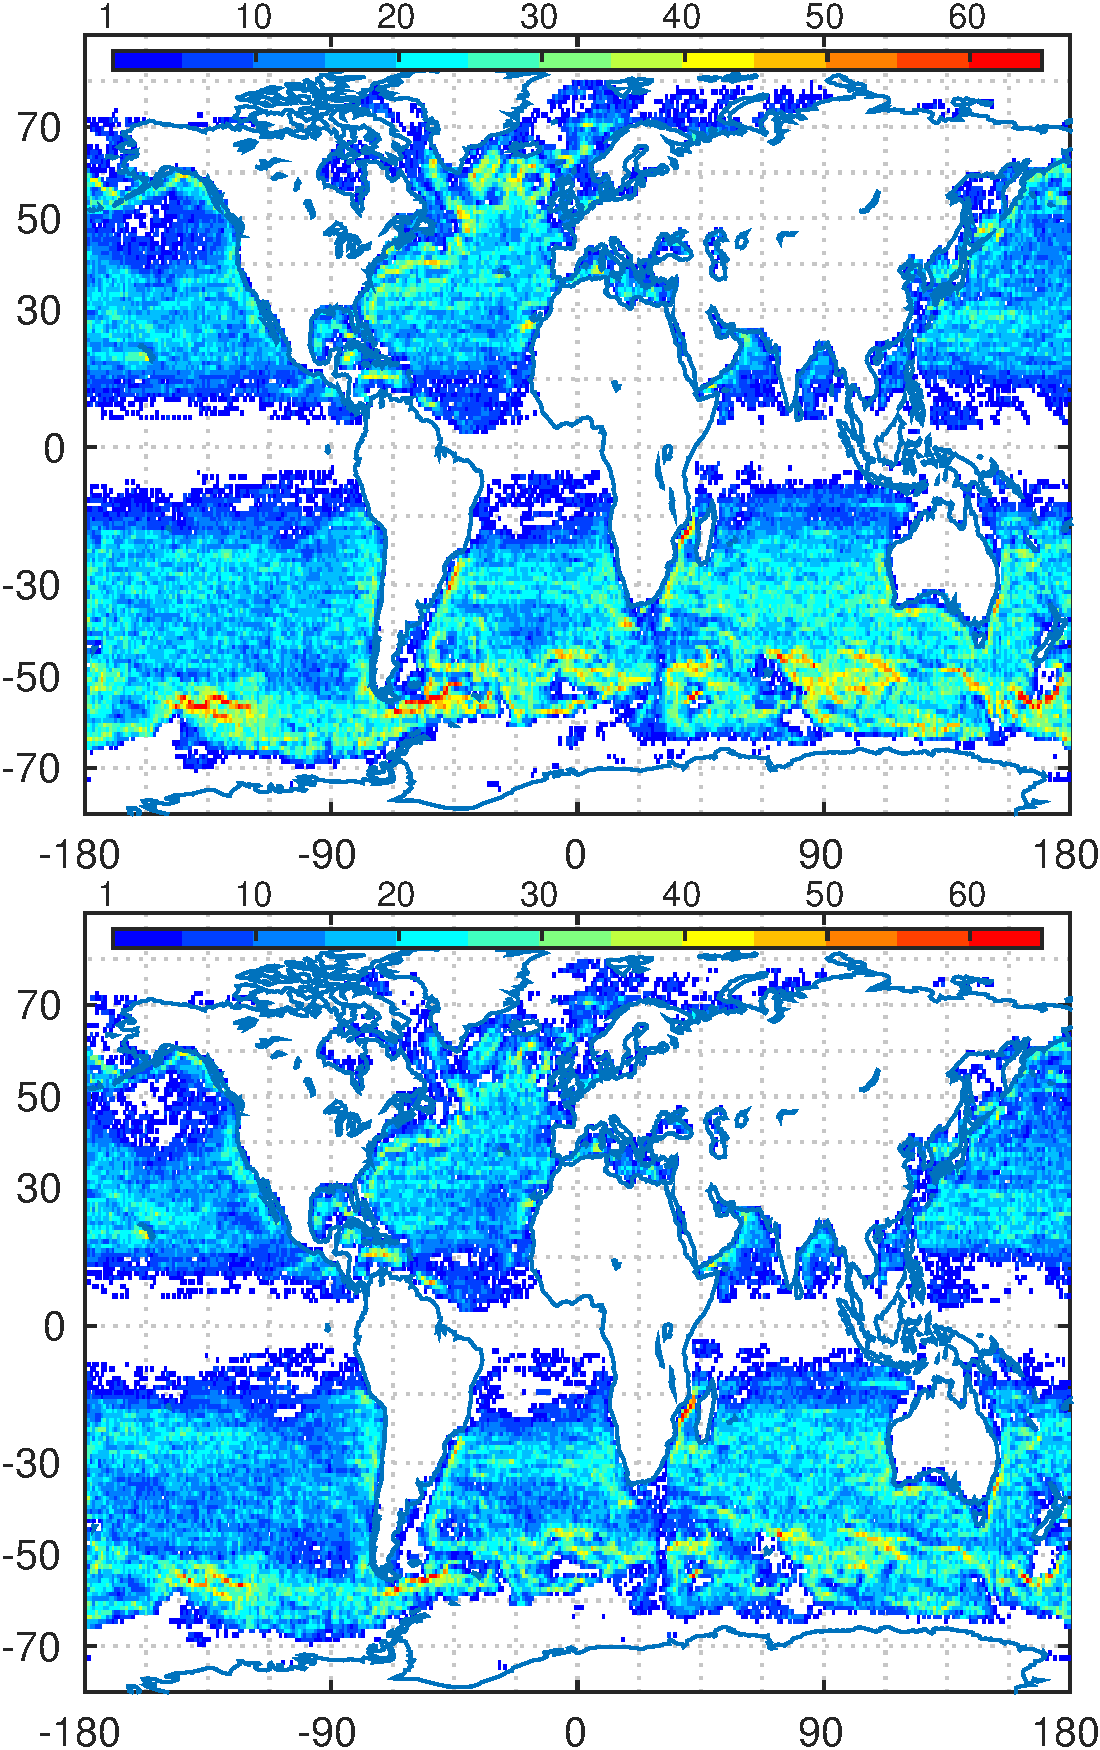
\includegraphics[width=1\linewidth]{MapVisitsBoth-aviIandaviII}
		\caption{Top: \aviI. Bottom: \aviII. Total count of individual eddies per 1 degree square.}
		\label{MapVisitsBoth-aviIandaviII}
\end{marginfigure}

%%%....................................F.I.G.U.R.E.............................................




%%....................................F.I.G.U.R.E.............................................
\begin{figure*}
		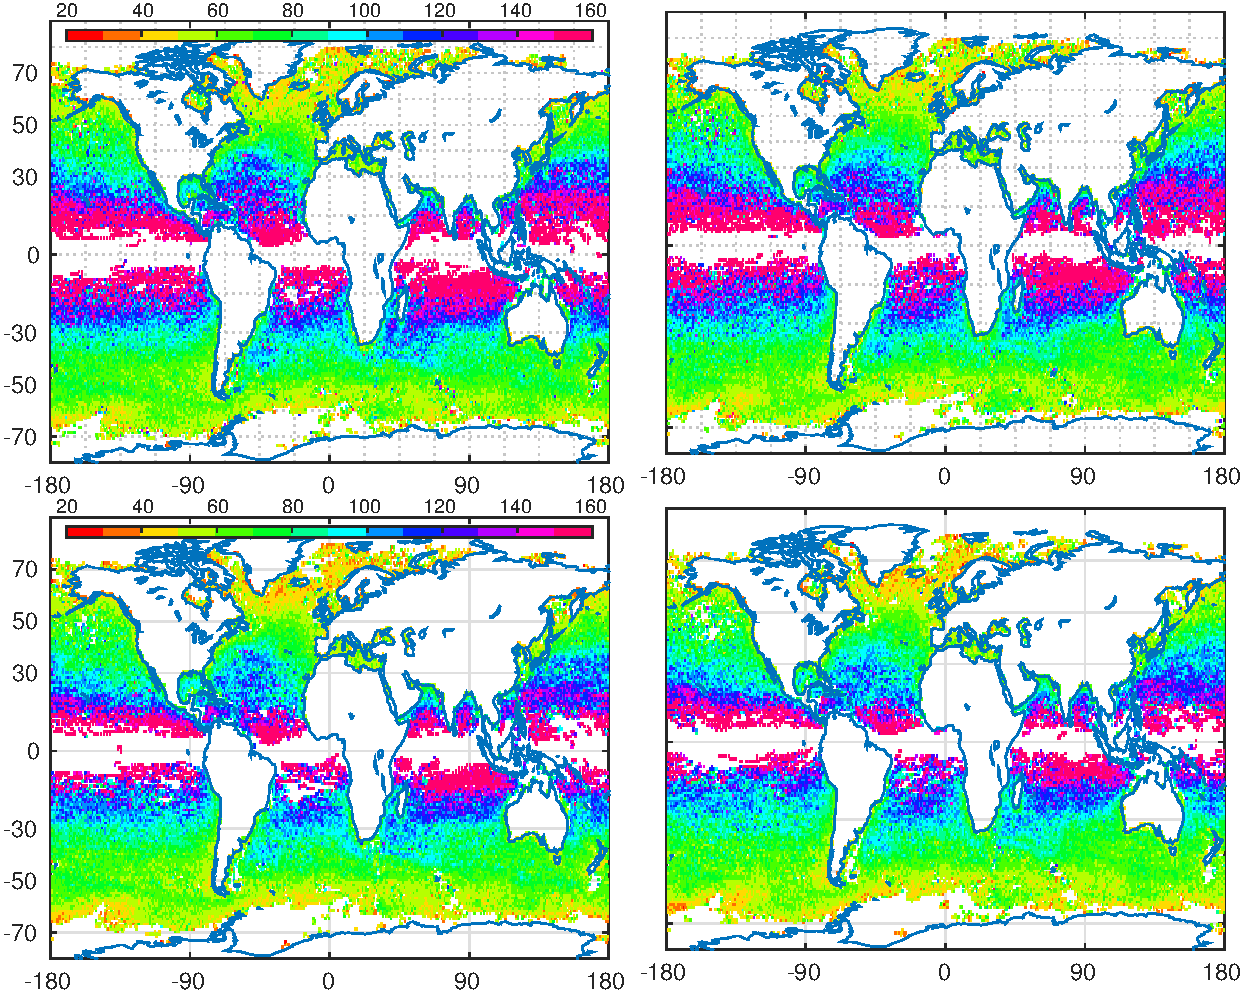
\includegraphics[]{sigmaAviBothItopIIbottom}
		\caption{Top: \aviI. Bottom \aviII. \capS}
	\label{fig:MapSigma-aviI}
\end{figure*}
%%....................................F.I.G.U.R.E.............................................

%%%....................................F.I.G.U.R.E.............................................
%\begin{figure*}
		%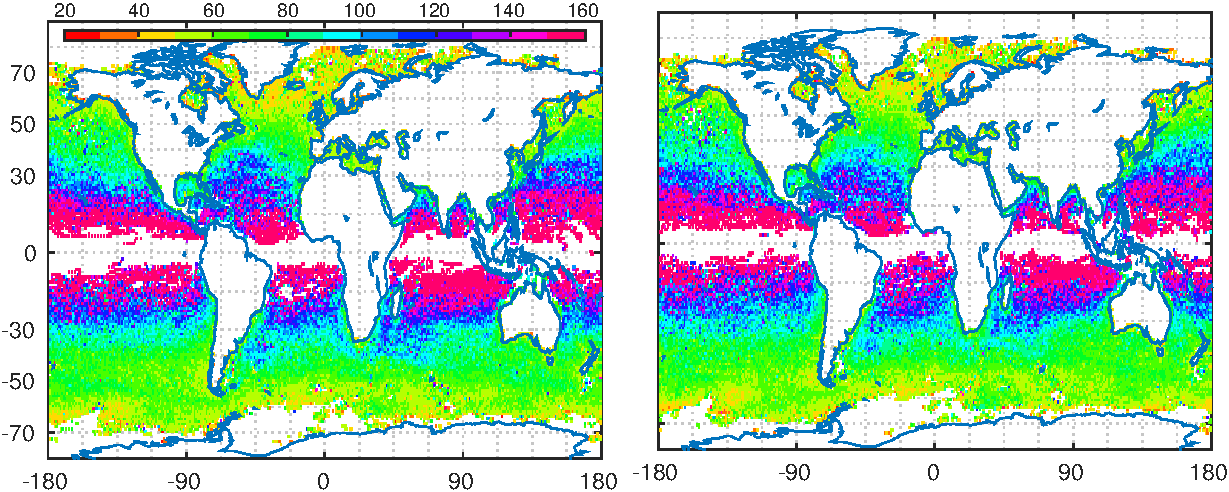
\includegraphics[]{MapSigma-aviI}
		%\caption{\aviI: \capS}
	%\label{fig:MapSigma-aviI}
%\end{figure*}
%%%....................................F.I.G.U.R.E.............................................

%%....................................F.I.G.U.R.E.............................................
\begin{figure*}
		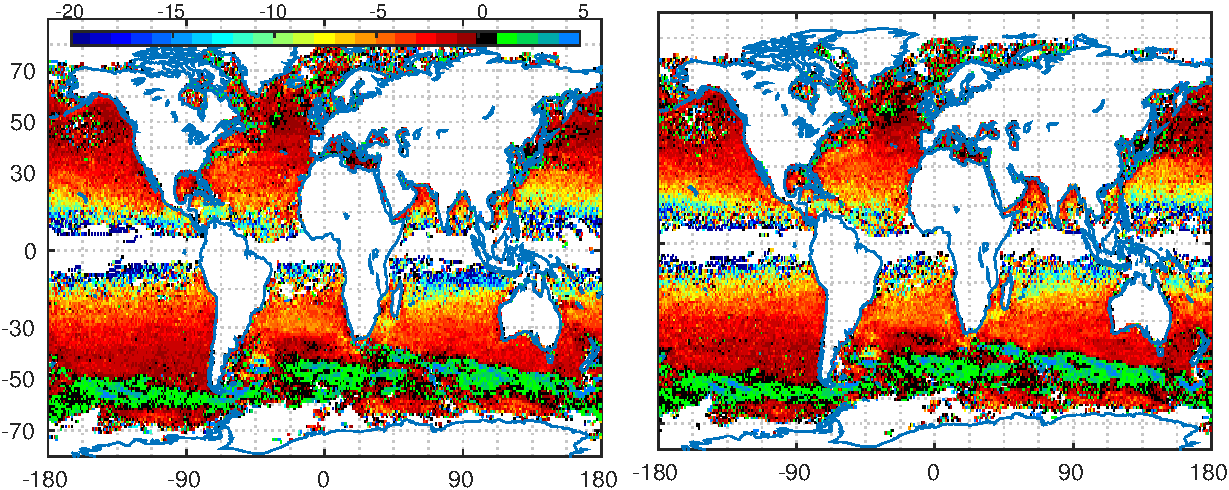
\includegraphics[]{velZon-aviI}
		\caption{\aviI: \capU. Respective map for \aviII not shown as it looks almost identical.}
	\label{fig:velZon-aviI}
\end{figure*}
%%....................................F.I.G.U.R.E.............................................
